\documentclass[12pt, titlepage]{article}
\usepackage{xcolor} % for different colour comments

%% Comments
\newif\ifcomments\commentstrue

\ifcomments
\newcommand{\authornote}[3]{\textcolor{#1}{[#3 ---#2]}}
\newcommand{\todo}[1]{\textcolor{red}{[TODO: #1]}}
\else
\newcommand{\authornote}[3]{}
\newcommand{\todo}[1]{}
\fi

\newcommand{\wss}[1]{\authornote{magenta}{SS}{#1}}
\newcommand{\ds}[1]{\authornote{blue}{DS}{#1}}

%% Graphics
\usepackage{float}
\usepackage{caption}
\usepackage{graphicx}
\usepackage{courier}
\graphicspath{ {images/} }

\begin{document}

\title{Smart Waiter User Guide} 
\author{Meraj Patel \#1137491 \\ Pavneet Jauhal \#1149311\\ Shan Perera \#1150394}
\date{\today}
\maketitle

\tableofcontents 

\listoffigures

\listoftables

\begin{table}[H]
\section*{Revision History}
\begin{tabular}{|c|c|}
\hline
\textbf{Date}  & \textbf{Comments} \\ \hline
February 29, 2016 &  first draft. \\ 
\hline
\end{tabular}
\caption{Revision History Table}
\end{table}

\section{Introduction}
\subsection{What is Smart-Waiter?}
\subsection{Objectives of User Manual}

\section{Getting Started }
\subsection{System Requirements}
\subsection{Installation Instructions}

\section{Account Setup}
\subsection{Creating an Account}
If this is the first time that Smart-Waiter is launched, you will be asked to create an account. You will be brought to the Account Creation screen as soon as Smart-Waiter is initialized. Your screen will look similar to Figure 1 below. 

\begin{center}
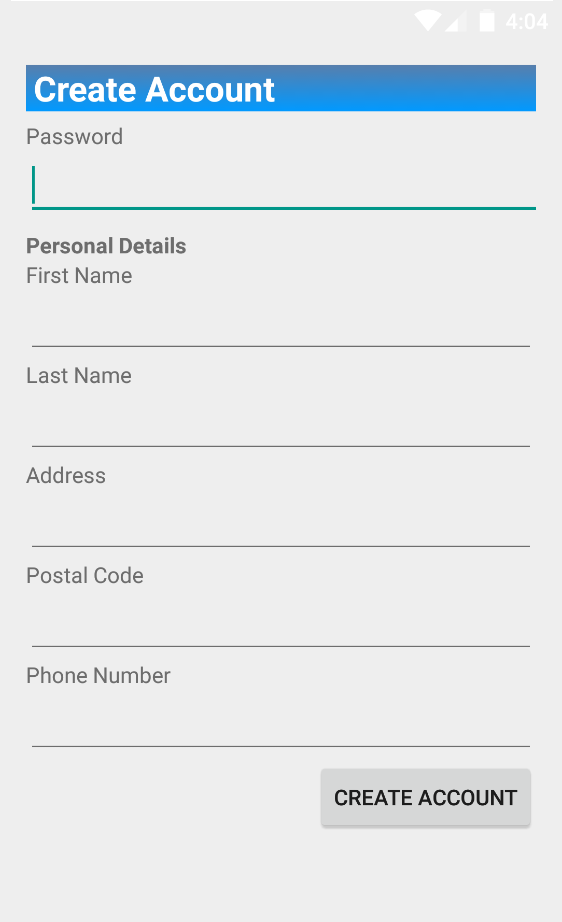
\includegraphics[width=0.5\textwidth]{accountCreation.png}
\linebreak Figure 1
\end{center}

The instructions to create an account are as follows: 
\begin{enumerate}
	\item Choose a password between 2-5 characters long.
	\item Enter your first name into the corresponding field.
	\item Enter your last name into the corresponding field.
	\item Enter the first line of your home address as it appears on your mail. Ex: \texttt{125 Royal Ave}
	\item Enter your postal code in the following format: \texttt{L4H 3Y4}
	\item Enter your phone number in the following format: \texttt{4165551911}
	\item Press the \texttt{Create Account} button.
\end{enumerate}

Your Smart-Waiter account has now been successfully created.
\subsection{Accessing Account Settings}
This feature is set to be implemented in our final revision. For the time being, a general walk-through is given using a generic android application settings module. To access your Account Settings in Smart-Waiter proceed with the following steps:

\begin{enumerate}
	\item Press the button with 3 horizontal white lines to bring up the 		Navigation menu, as seen in Figure 2: 
	\begin{center}
	
\includegraphics[width=0.05\textwidth]{ui-fragment-button.png}
	\linebreak Figure 2
	\end{center}

	\item Press the \texttt{Settings} button in the Navigation Menu as seen 	in Figure 3:
	\begin{center}
	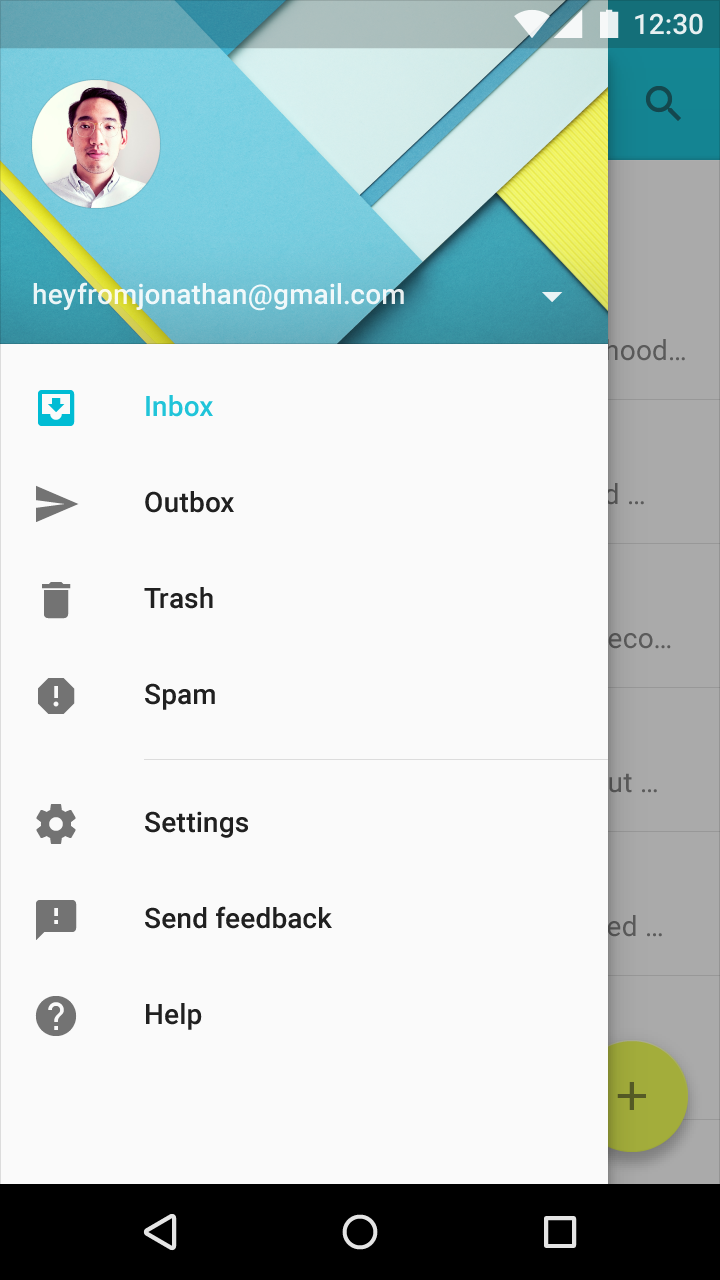
\includegraphics[width=0.4\textwidth]{nav-menu.png}
	\linebreak Figure 3
	\end{center}
\end{enumerate}

From here you can edit your Account Settings. You can perform the following actions in the settings page: \texttt{Change Password} and \texttt{Edit Personal Details}.

\textbf{Changing Your Password:}
	\begin{enumerate}
		\item Press the \texttt{Change Password} label.
		\item Enter your current password into the corresponding field
		\item Press the \texttt{Confirm} button
		\item Enter a new password between 2-5 characters
		\item Enter your new password again into the \texttt{Confirm Password} field
		\item Press the \texttt{Update Password} button.
	\end{enumerate}
	
\textbf{Editing Your Personal Details:}
	\begin{enumerate}
		\item Press the \texttt{Edit Personal Details} label.
		\item Enter your updated information into the corresponding field
		\begin{enumerate}
			\item \textbf{NOTE:} If you leave a field blank, the 						information for the corresponding field will not be updated.
		\end{enumerate}
		\item Press the \texttt{Save Changes} button.
	\end{enumerate}
\section{View Restaurant Menu}
\subsection{Scanning Barcode}
\subsection{Menu Layout}

\section{Placing an Order}
\subsection{Adding Item to Cart}
\subsection{Confirmation and Payment}
\subsection{Submitting an Order}

\section{Troubleshooting}
\subsection{Overview}
\subsection{Barcode Scanning Error}
\subsection{Application Freeze}
\subsection{Frequently Asked Questions}



\end{document}